\documentclass[12pt]{article}
\setlength{\oddsidemargin}{0.0in} \setlength{\evensidemargin}{0.0in}
\setlength{\textwidth}{6.5in} \setlength{\topmargin}{-0.25in}
\setlength{\textheight}{8.75in}
\usepackage{amsmath, amssymb, amsfonts, amsthm, amscd, xspace, pifont, natbib, fullpage, enumitem, bm, bbm}
\usepackage{fullpage}
\usepackage{graphicx, float}
\usepackage{epsfig, amsfonts, verbatim, multirow, hyperref}
\usepackage{epstopdf}
\usepackage{listings, boxedminipage}

\lstset{
	basicstyle=\ttfamily,
	mathescape
}
%\usepackage{setspace}
\newcommand{\mycite}[1]{{\citeNP{#1}}}

\parindent=0pt

%%%%%%%%%%%%%%%%%%%%%%%%%%%%%%%%%%%%%%%%%%%%%%%%%%%%%%%%%%%%%%%%%%%%%%%%%%%%%%%%%%%%%%%%%%%%%%%%%%%
% Different font in captions
\newcommand{\captionfonts}{\small}
\makeatletter  % Allow the use of @ in command names
\long\def\@makecaption#1#2{%
	\vskip\abovecaptionskip
	\sbox\@tempboxa{{\captionfonts #1: #2}}%
	\ifdim \wd\@tempboxa >\hsize
	{\captionfonts #1: #2\par}
	\else
	\hbox to\hsize{\hfil\box\@tempboxa\hfil}%
	\fi
	\vskip\belowcaptionskip}
\makeatother   % Cancel the effect of \makeatletter
%%%%%%%%%%%%%%%%%%%%%%%%%%%%%%%%%%%%%%%%%%%%%%%%%%%%%%%%%%%%%%%%%%%%%%%%%%%%%%%%%%%%%%%%%%%%%%%%%%%

%% Matrix, Vector
\newcommand{\V}[1]{\ensuremath{\boldsymbol{#1}}\xspace}
\newcommand{\M}[1]{\ensuremath{\boldsymbol{#1}}\xspace}
%% Math Functions
\newcommand{\F}[1]{\ensuremath{\mathrm{#1}}\xspace}
\newcommand{\sgn}{\F{sgn}}
\newcommand{\tr}{\F{trace}}
\newcommand{\diag}{\F{diag}}
\newcommand{\dett}{\F{det}}
%% Transpose
\newcommand{\T}[1]{\ensuremath{{#1}^{\mbox{\sf\tiny T}}}}

%%
\def  \R  {\boldsymbol R}
\def\bX{\boldsymbol X}
\def\bY{\boldsymbol Y}
\def\bbeta{\boldsymbol \beta}
\def\blambda{\boldsymbol \lambda}
\def\bepsilon{\boldsymbol \epsilon}
\def\bone{\boldsymbol{1}}
\def\bzero{\boldsymbol 0}
\def\E{\mbox{E}}
\def\var{\mbox{var}}
\def\gauss{\mbox{N}}
\def\lap{\mbox{L}}
\def\G{\mbox{G}}
\def\go{  $\R$  ightarrow}
\def\invG{\mbox{G}^{-1}}
\def\argmin{\arg\min}

\newtheorem{theorem}{Theorem}
\newtheorem{proposition}{Proposition}
\newtheorem{lemma}{Lemma}
\newtheorem{corollary}{Corollary}
\newtheorem{algorithm}{Algorithm}
\newtheorem{definition}{Definition}
\newtheorem{remark}{Remark}

\usepackage{color}
\definecolor{codegreen}{rgb}{0,0.6,0}
\definecolor{codegray}{rgb}{0.5,0.5,0.5}
\definecolor{codepurple}{rgb}{0.58,0,0.82}
\definecolor{backcolour}{rgb}{0.95,0.95,0.92}
\lstdefinestyle{displaycode}{
	backgroundcolor=\color{backcolour},   
	commentstyle=\color{codegreen},
	keywordstyle=\color{magenta},
	numberstyle=\tiny\color{codegray},
	stringstyle=\color{codepurple},
	basicstyle=\footnotesize,
	breakatwhitespace=false,         
	breaklines=true,                 
	captionpos=b,                    
	keepspaces=true,                 
	columns=flexible,
	numbers=none,
	numbersep=5pt,                  
	showspaces=false,                
	showstringspaces=false,
	showtabs=false,                  
	tabsize=2%,
	%xleftmargin=2em,
	%xrightmargin=2em,
} 
\lstdefinestyle{displaycode2}{
	backgroundcolor=\color{backcolour},   
	commentstyle=\color{red},
	keywordstyle=\color{magenta},
	numberstyle=\tiny\color{codegray},
	stringstyle=\color{codepurple},
	basicstyle=\footnotesize,
	breakatwhitespace=false,         
	breaklines=true,                 
	captionpos=b,                    
	keepspaces=true,                 
	columns=flexible,
	numbers=none,
	numbersep=5pt,                  
	showspaces=false,                
	showstringspaces=false,
	showtabs=false,                  
	tabsize=2%,
	%xleftmargin=2em,
	%xrightmargin=2em,
} 

\lstset{style=displaycode}
%\newcommand{\displaycodefile}[1]{\lstinputlisting[language=R]{./codeblocks/#1.txt}}

\newcommand{\pr}{\mathbb{P}}

\renewcommand{\thefootnote}{\fnsymbol{footnote}}

\begin{document}
\title{\Large \bf STATS 406 F15: Lab 06\\
	Importance sampling}
\date{}

\maketitle

\underline{Disclaimer: This note uses its own notation. Do not make direct notational match with lecture notes.}

\section{Scenarios where naive Monte Carlo Integration is a poor choice}

\begin{itemize}
	\item \underline{Example 1}\footnote{Section 2.5.1, ``\emph{Monte Carlo Strategies in Scientific Computing}'' by Jun Liu}
	{\bf (Locally concentrated integrand)}\\
	Consider the following function:
	$$
	f(x, y) :=  0.5 e^ {-90 (x-0.5)^2-45 (y+0.1)^4}  +  e^{-45 (x+0.4)^2-60 (y-0.5)^2}
	$$
	{\bf Goal:} compute
	$$
	I_1 := \int_{-1}^1\int_{-1}^1 f(x, y) \textrm{d}x\textrm{d}y
	$$
\begin{lstlisting}[style=displaycode2, language=Mathematica]
(* Illustration: see Lab_5.nb (in Mathematica) *)
\end{lstlisting}

	\item \underline{Example 2} {\bf (High-dimensional integration)}\\
	For a $p$-dimensional variable $\bm{x}:=(x_1, \ldots, x_p)^T\in\mathbb{R}^p$ and a funciton $f:\mathbb{R}^p\to\mathbb{R}$, consider the integral:
	$$
	I_2:= \int_{[-1,1]^p} f(\bm{x})\mathbbm{1}[\|\bm{x}\|_2\leq 1] \textrm{d}\bm{x}
	$$
	Here, the integrand $f(\bm{x})\mathbbm{1}[\|\bm{x}\|_2\leq 1]$ is only non-zero inside the $p$-dimensional unit ball: ${\cal B}^p:=\{\bm{x}: \|\bm{x}\|_2\leq 1\}$.
	\begin{itemize}[label=*]
		\item If we follow the naive Monte Carlo integration, in which we sample $\bm{x}$ by uniformly sampling each of its element $x_i$ from Unif$[-1, 1]$, that is, sampling uniformly from the $p$-dimensional unit cube ${\cal C}^p:=\{ \bm{x}: \|\bm{x}\|_\infty\leq 1 \}$, what will happen?
		\item {\bf Volume of the $p$-dimensional unit cube ${\cal C}^p$:}
		$$
		\textrm{Volume}({\cal C}^p) = 2^p
		$$
		\item {\bf Volume of the $p$-dimensional unit ball ${\cal B}^p$:}
		$$
		\textrm{Volume}({\cal B}^p) = \frac{\left(\sqrt{\pi}\times 1\right)^p}{\Gamma\left(\frac{p}{2}+1\right)} \stackrel{\textrm{large }p}{\sim} \frac{1}{\sqrt{p\pi}}\left(\frac{2\pi e}{p}\right)^{\frac{p}{2}} 1^p = \textrm{Constant}\times p^{-\frac{p+1}{2}}
		$$
		where the first approximation is by Stirling's formula.
		\item \textcolor{red}{\bf The proportion of ``wasted'' sample points goes lightning fast to 100\% as $p$ increases!}
		\item The ``curse of dimensionality'': the` sample size needed increses exponentially with the dimension.
	\end{itemize}
\end{itemize}



\section{Importance sampling(primary form)}
Importance sampling is a representative technique for carrying out Monte Carlo integration.
\begin{itemize}
	\item {\bf Goal:} compute $I=\int f(\bm{x})\textrm{d}\bm{x}$. In examples we saw last week, $\bm{x}=x$ is a scalar(1-dimensional); in \underline{Example 1}, $\bm{x}=(x, y)$ is 2-dimensional; in \underline{Example 2}, $\bm{x}\in\mathbb{R}^p$.
	\item A general approach is to choose a distribution $\pi(\bm{x})$ and rewrite
	$$
	I = \int f(\bm{x})\textrm{d}\bm{x} = \int \frac{f(\bm{x})}{\pi(\bm{x})} \cdot \pi(\bm{x})\textrm{d}\bm{x} = \mathbb{E}\left[ \frac{f(\bm{X})}{\pi(\bm{X})} \right]
	$$
	Thus a natural estimator for $I$ is therefore
	\begin{equation}
	\hat{I}:=\hat{\mathbb{E}}\left[ \frac{f(\bm{x})}{\pi(\bm{x})} \right] = \frac{1}{n}\left\{ \frac{f(\bm{X_1})}{\pi(\bm{X_1})}, \ldots, \frac{f(\bm{X_n})}{\pi(\bm{X_n})} \right\}   \label{Ihat}
	\end{equation}
	where $\bm{X}_i\stackrel{\textrm{PDF}}{\sim}\pi(\bm{x})$.
	\item $\hat{I}$ is always an \textcolor{blue}{unbiased} estimator of $I$ regardless of the choice of $\pi$, in the sense that
	$$
	\mathbb{E}[\hat{I}] = \mathbb{E}\left[ \frac{f(\bm{X})}{\pi(\bm{X})} \right]
	$$
	Good and bad choices of $\pi$ are differentiated by the ``stability'' of the resulting estimator $\hat{I}$, mathematically described by $\textrm{Var}\left[ \hat{\mathbb{E}}\left[ \frac{f(\bm{X})}{\pi(\bm{X})} \right] \right]$.
	\item {\bf How to choose a good $\pi$?}\\
	For simplicity, define $\mu:=\mathbb{E}\left[ \frac{f(\bm{X})}{\pi(\bm{X})} \right] = \int f(\bm{x})\textrm{d}\bm{x}$. Now we show how to choose $\pi$ to minimize the variance. Notice
	\begin{align*}
	\textrm{Var}\left( \frac{f(\bm{X})}{\pi(\bm{X})} \right) &= \int\left\{ \frac{f(\bm{x})}{\pi(\bm{x})} - \mu \right\}^2 \pi(\bm{x}) \textrm{d}\bm{x} = \int\left\{ \frac{f^2(\bm{x})}{\pi(\bm{x})} - 2f(\bm{x})\mu + \mu^2\pi(\bm{x}) \right\}\textrm{d}\bm{x}\\
	&=\int \frac{f^2(\bm{x})}{\pi(\bm{x})}\textrm{d}\bm{x}  - \mu^2
	\end{align*}
	Since $\pi$ is a density,
	$$
	\int \pi(\bm{x})\textrm{d}\bm{x}=1
	$$
	By Cauchy-Schwartz inequality, we have
	$$
	\left(\int \frac{f^2(\bm{x})}{\pi(\bm{x})}\textrm{d}\bm{x}\right)\left(\int \pi(\bm{x})\textrm{d}\bm{x}\right) \geq \left( \int f(\bm{x})\textrm{d}\bm{x} \right)^2
	$$
	where equality holds only when
	$$
	\frac{f^2(\bm{x})}{\pi(\bm{x})} \Big/ \pi(\bm{x}) = \textrm{Constant}
	$$
	Therefore, the best choice of $\pi$ is
	$$
	\pi(\bm{x})\propto f(\bm{x})
	$$
	\item In practice, we do not always know how to sample from a $\pi(\bm{x})$ that follows the shape of $f(\bm{x})$, but we usually can find a $\pi$ whose shape is similar to $f$, and such $\pi$ is usually a decent choice.
\end{itemize}



\section{Revisit Examples 1 and 2 with importance sampling}

\underline{Example 1}

\begin{itemize}
	\item Telling from visual, we should choose $\pi(x, y)$ to be a (truncated) mixture of 2-dimensional normal distributions, with a shape similar to $f(x, y)$.
	\item We approximately express $f$ to be proportional to a mixture of normal distributions. In order to do this we first approximate $e^{-(y+0.1)^4}$ with $e^{-10(y+0.1)^2}$:
	\begin{figure}[H]
		\centering
		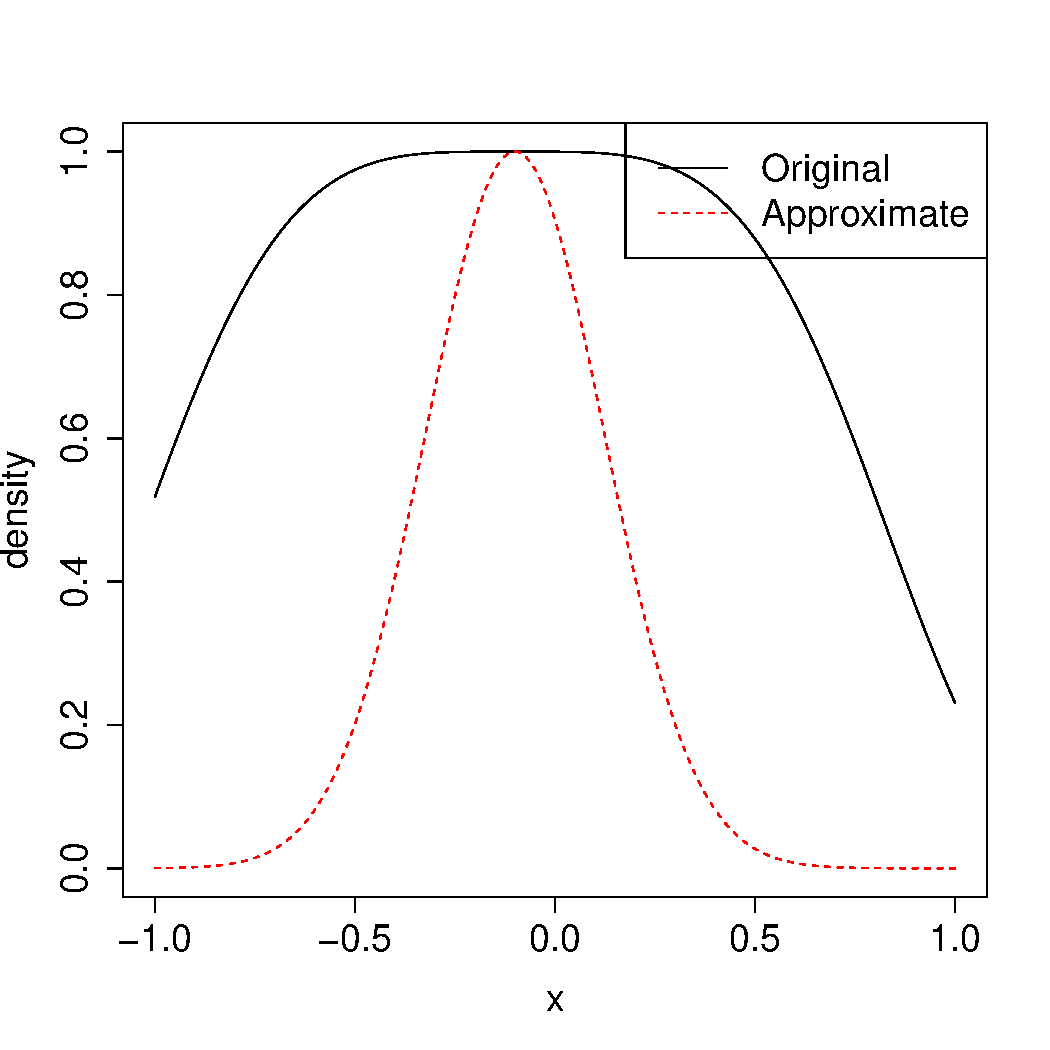
\includegraphics[width=0.5\textwidth]{illustration.pdf}
	\end{figure}
	rewrite
	\begin{align}
		f(x, y) &\approx 0.5 e^ {-90 (x-0.5)^2 - 10 (y+0.1)^2}  +  e^{-45 (x+0.4)^2-60 (y-0.5)^2}\nonumber\\
		 &= 0.5 \times \exp \left[ - \left\{ \frac{(x-0.5)^2}{2\times \frac{1}{180}} + \frac{(y+0.1)^2}{2\times \frac{1}{20}} \right\} \right]\nonumber\\
		 &+ 1\times \exp\left[ -\left\{ \frac{(x+0.4)^2}{2\times\frac{1}{90}} + \frac{(y-0.5)^2}{2\times\frac{1}{120}} \right\} \right]\nonumber\\
		 &\propto 0.464 \times {\cal N}\left[ \begin{pmatrix} 0.5\\ -0.1
		 \end{pmatrix}, \begin{pmatrix} \frac{1}{180} & 0\\ 0 & \frac{1}{20} \end{pmatrix} \right]
		 + 0.536 \times {\cal N}\left[ \begin{pmatrix} -0.4\\ 0.5
		 \end{pmatrix}, \begin{pmatrix} \frac{1}{90} & 0\\ 0 & \frac{1}{120} \end{pmatrix} \right]    \label{GaussianMixture}
	\end{align}
	Therefore, in the importance sampling, we should choose $\pi(\bm{x})$ as follows:
	$$
	\pi(\bm{x}) = \pi(x, y)
	\begin{cases}
	\propto \textrm{PDF of RHS of \eqref{GaussianMixture}} & \textrm{if }(x, y) \in [-1, 1]^2\\
	=0 & \textrm{otherwise}
	\end{cases}
	$$
	\item We have the following algorithm to sample from $\pi(\bm{x})$:
	\begin{enumerate}
		\item Toss a coin with probability $0.464$ to sample from the first normal distribution and with probability $0.536$ to sample from the second normal distribution.
		\item Sample $\bm{X}=(X, Y)$ from the chosen multivariate normal distribution
		\item Accept $\bm{X}=(X, Y)$ if it falls within $[-1, 1]^2$, otherwise reject it and return to Step 1.
	\end{enumerate}
	\item Then estimate $I$ by $\hat{I}$ defined in \eqref{Ihat}.
\end{itemize}
\begin{lstlisting}[style=displaycode, language=R]
# Numerical experiments for Example 1: see Lab_5.R
\end{lstlisting}


\underline{Example 2}

\begin{itemize}
	\item The choice of $\pi(\bm{x})$ depends on the shape of $f(\bm{x})$. For example, choosing $\pi(\bm{x})$ to be a multivariate normal distribution usually alleviates (but may not completely remedy) the curse of dimensionality.
\end{itemize}

\section{A useful variant estimator(reviewing lecture content)}
\begin{itemize}
	\item {\bf Beginning of the story -- a slightly different goal:} Now we want to evalute $\mathbb{E}[g(\bm{X})]$, where the random variable $\bm{X}\stackrel{\textrm{PDF}}{\sim} p(\bm{x})$.	Written in integration form:
	\begin{equation}
	J := \int g(\bm{x}) p(\bm{x}) \textrm{d}\bm{x}   \label{Goal2}
	\end{equation}
	\item If the shape of $g(\bm{x})$ suggests that an importance sampling is needed and we know the exact $p(\bm{x})$, we can choose a proper density $q(\bm{x})$, and rewrite $J$:
	$$
	J := \int g(\bm{x}) p(\bm{x}) \textrm{d}\bm{x} = \int \frac{g(\bm{x}) p(\bm{x})}{q(\bm{x})} \times q(\bm{x})\textrm{d}\bm{x} = \mathbb{E}\left[ \frac{g(\bm{X}) p(\bm{X})}{q(\bm{X})} \right]
	$$
	Then compute the estimator (similar to \eqref{Ihat})
	\begin{equation}
	\hat{J} := \frac{1}{n}\left\{ \frac{g(\bm{X_1}) p(\bm{X_1})}{q(\bm{X_1})} + \ldots + \frac{g(\bm{X_n}) p(\bm{X_n})}{q(\bm{X_n})} \right\}   \label{Jhat}
	\end{equation}
	where $\bm{X}_i\stackrel{\textrm{PDF}}{\sim}q(\bm{x})$.
	\item But sometimes, we only know $p(\bm{x})$ up to a normalizing constant, i.e. $p(\bm{x}) = C\times p_0(\bm{x})$.
	\begin{itemize}[label=*]
		\item A familiar example: $p(\bm{x})$ is a truncated normal distribution.
		\item A more realistic-like (though still artificial) example:
		\begin{enumerate}
			\item Define random variable $\bm{U}:=(U_1, \ldots, U_p)\in\{0,1\}^p$.
			\item $U_k$'s are independent, $U_k\sim$Bernoulli$(v_k)$, $k=1,\ldots,p$.
			\item Given $\bm{U}$, $\bm{x}$ follows a conditional distribution $p(\bm{x}|\bm{U})$.
			\item Obviously,
			$$
			p(\bm{x}) \propto \sum_{u_1,\ldots,u_p\in\{0,1\}^p} \left[ p(\bm{x}|\bm{u}) \times \prod_{k=1}^p\left\{ u_k^{v_k}(1-u_k)^{1-v_k}\right\} \right]
			$$
			\item When $p$ is large, it is computationally infeasible to enumerate all possibilities for $\bm{u}\in\{0,1\}^p$, which is necessary for computing the normalizing constant in $p(\bm{x})$.
		\end{enumerate}
		\item \textcolor{red}{Now we don't know the normalizing constant in $p(\bm{x})$, the problem \eqref{Goal2} becomes different from the problem ``compute an integral by Monte Carlo methods'', because the integrand is not fully specified.}
	\end{itemize}
	Notice that \eqref{Jhat} requires the knowledge of the normalizing constant (must know exact $p(\bm{x})$) and is thus inapplicable here.
	\item {\bf A useful variant of \eqref{Jhat}}\\
	Consider $\tilde{J}$, in which we are only allowed to use $p_0$, not $p$, as follows:
	\begin{equation}
	\tilde{J}:=\dfrac{\dfrac{g(\bm{X_1}) p_0(\bm{X_1})}{q(\bm{X_1})} + \ldots + \dfrac{g(\bm{X_n}) p_0(\bm{X_n})}{q(\bm{X_n})}}{\dfrac{p_0(\bm{X_1})}{q(\bm{X_1})} + \ldots + \dfrac{p_0(\bm{X_n})}{q(\bm{X_n})}}   \label{Jtilde}
	\end{equation}
	where $\bm{X}_i\stackrel{\textrm{PDF}}{\sim}q(\bm{x})$. Obviously, apart from the difference in $p$ and $p_0$, $\hat{J}$ just amounts to replace the denominator of $\tilde{J}$ by $n$.
	\begin{itemize}[label=*]
		\item {\bf Advantage of \eqref{Jtilde}}: it suffices to know $p_0(\bm{x})$, since $C$ in the numerator and the denominator cancel out.
		\item {\bf Asymptotic unbiasedness of $\tilde{J}$:}
		\begin{enumerate}
			\item {\bf The numerator:} by Strong Law of Large Numbers,
			\begin{equation}
			\left\{\dfrac{g(\bm{X_1}) p_0(\bm{X_1})}{q(\bm{X_1})} + \ldots + \dfrac{g(\bm{X_n}) p_0(\bm{X_n})}{q(\bm{X_n})}\right\}\Big/ n \stackrel{\textrm{a.s.}}{\to} \mathbb{E}\left[ \frac{g(\bm{X}) p(\bm{X})}{q(\bm{X})} \right] =: J   \label{Denominator}
			\end{equation}
			\item {\bf The denominator:} by Strong Law of Large Numbers,
			\begin{equation}
			\left\{ \dfrac{p_0(\bm{X_1})}{q(\bm{X_1})} + \ldots + \dfrac{p_0(\bm{X_n})}{q(\bm{X_n})} \right\}\Big/ n \stackrel{\textrm{a.s.}}{\to} \mathbb{E}\left[ \frac{p(\bm{X})}{q(\bm{X})} \right] = \int \frac{p(\bm{x})}{q(\bm{x})}q(\bm{x})\textrm{d}\bm{x} = \int p(\bm{x})\textrm{d}\bm{x} = 1   \label{Numerator}
			\end{equation}
			\item Divide the numerator and denominator of the RHS of \eqref{Jtilde} by $n$ and apply \eqref{Denominator}
 and \eqref{Numerator}. By Slutsky's theorem:\\
			 \url{https://en.wikipedia.org/wiki/Slutsky\%27s_theorem}\footnote{We used the a.s. convergence version Slutsky's theorem, which is not shown in the Wiki page but can be proved similarly with the continuous mapping theorem.},
			 we have
			 $$
			 \tilde{J}\stackrel{\textrm{a.s.}}{\to} J
			 $$
			 as $n\to\infty$.
		 \end{enumerate}
	\end{itemize}
\end{itemize}









\end{document}